% Nallino, Part I p. 180: the figure of the gnomon and its shadow, redrawn from the print: the gnomon AB, the
% shadow CB (umbra extensa) and the ray AC as solid lines; the line DGA, the sine GF, the ray produced CF and
% the line BE in dashes; the quadrant DFE about A in dashes; the angle h at A and at C; the braces of cos h,
% sin h and p; the italic letters and words. Measured on the scan (_intake/latin/tools/fig180).
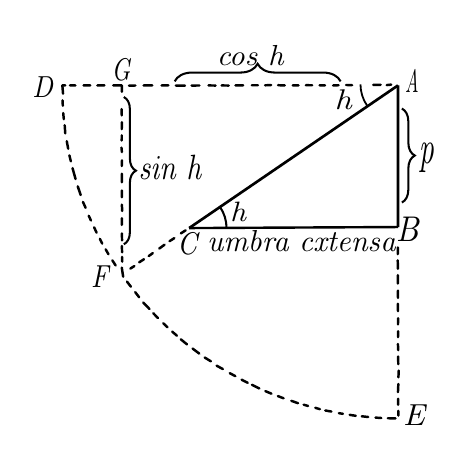
\begin{tikzpicture}[x=0.9928pt,y=-0.9928pt,line cap=butt,every node/.style={font=\fontsize{11}{11}\bfseries\itshape\selectfont,inner sep=0pt}]
\useasboundingbox (0,0) rectangle (143.00,146.00);
\draw[line width=0.95pt] (134.79,21.01) -- (134.80,72.56);  % the gnomon AB
\draw[line width=0.87pt] (58.77,72.94) -- (134.80,72.56);  % the shadow CB
\draw[line width=0.96pt] (134.79,21.01) -- (58.77,72.94);  % the ray AC
\draw[line width=0.65pt] (123.54,28.37) arc[start angle=145.47,end angle=180.00,radius=13.66];
\draw[line width=0.74pt] (69.98,65.23) arc[start angle=-34.53,end angle=0.00,radius=13.61];
% the dashes of DGA, GF, CF, BE and of the quadrant DFE, each where it printed
\draw[line width=0.89pt,line cap=round] (115.88,20.86)--(118.09,20.92) (125.77,20.81)--(128.46,20.79) (130.68,20.90)--(132.32,20.72) (15.39,20.98)--(17.36,21.02) (20.32,21.04)--(22.77,20.99) (48.76,21.04)--(51.21,20.99) (75.63,21.03)--(78.44,20.98) (81.60,20.96)--(83.80,20.96);
\draw[line width=0.89pt,line cap=round] (86.40,20.97)--(88.61,20.90) (91.12,20.94)--(93.57,21.02) (96.49,21.01)--(98.58,20.97) (101.23,20.94)--(103.55,20.96) (25.36,21.04)--(27.93,20.99) (31.12,21.01)--(34.29,21.01) (34.29,21.01)--(34.29,23.30) (36.89,21.08)--(39.21,21.05);
\draw[line width=0.89pt,line cap=round] (42.20,21.01)--(45.36,21.02) (53.94,21.06)--(57.23,21.10) (59.69,21.06)--(62.49,21.05) (65.81,21.03)--(68.38,21.06) (70.61,21.03)--(73.18,21.06) (106.25,20.98)--(108.21,21.00) (111.17,21.02)--(113.15,20.95) (134.77,80.00)--(134.70,82.46);
\draw[line width=0.89pt,line cap=round] (134.68,84.70)--(134.76,87.75) (134.72,90.08)--(134.76,93.13) (134.77,95.69)--(134.78,98.37) (134.77,100.49)--(134.78,103.17) (134.84,105.78)--(134.78,108.00) (134.84,110.51)--(134.79,112.60) (134.76,115.14)--(134.86,117.36) (134.83,119.69)--(134.89,122.49);
\draw[line width=0.89pt,line cap=round] (135.05,124.81)--(134.94,127.26) (134.91,129.69)--(134.77,132.63) (134.86,135.06)--(134.86,137.26) (134.89,139.45)--(134.94,141.18) (34.19,29.64)--(34.24,31.96) (34.28,34.39)--(34.24,36.96) (34.24,39.22)--(34.23,41.07) (34.14,43.66)--(34.29,45.28);
\draw[line width=0.89pt,line cap=round] (34.33,48.26)--(34.24,50.35) (34.28,53.13)--(34.30,56.29) (34.28,59.26)--(34.28,61.70) (34.28,64.41)--(34.41,66.72) (34.28,69.34)--(34.28,71.78) (34.29,74.87)--(34.35,77.44) (34.30,79.43)--(34.35,81.76) (34.37,83.42)--(34.40,85.15);
\draw[line width=0.89pt,line cap=round] (57.50,73.76)--(55.76,74.87) (53.37,76.60)--(51.63,77.72) (49.81,79.00)--(47.89,80.39) (45.55,82.05)--(44.06,83.12) (42.33,84.28)--(40.59,85.40) (38.83,86.76)--(37.36,87.69) (34.25,87.33)--(34.75,90.64) (12.62,21.01)--(13.68,21.01);
\draw[line width=0.89pt,line cap=round] (12.62,21.01)--(12.87,24.02) (12.68,26.43)--(12.79,28.41) (12.94,31.07)--(13.15,33.31) (13.47,35.51)--(13.68,38.46) (14.23,41.32)--(14.74,44.06) (15.18,46.47)--(15.72,48.65) (16.33,51.13)--(17.43,55.10) (18.22,57.75)--(19.29,60.93);
\draw[line width=0.89pt,line cap=round] (20.12,63.43)--(21.09,65.57) (22.20,68.46)--(23.04,70.18) (24.19,72.67)--(25.08,74.62) (26.28,76.86)--(27.12,78.58) (28.38,80.68)--(29.40,82.45) (30.82,84.69)--(32.02,86.55) (36.14,92.42)--(37.57,94.28) (39.14,96.26)--(40.57,98.12);
\draw[line width=0.89pt,line cap=round] (42.07,100.04)--(44.32,102.38) (45.71,103.94)--(47.46,105.71) (49.35,107.59)--(50.91,109.07) (52.59,110.63)--(54.31,112.10) (55.73,113.43)--(58.00,115.27) (60.02,116.80)--(62.46,118.61) (64.43,120.06)--(66.68,121.43) (68.77,123.02)--(71.03,124.25);
\draw[line width=0.89pt,line cap=round] (73.56,125.74)--(75.58,126.84) (77.87,128.12)--(80.10,129.25) (81.63,130.00)--(84.32,131.31) (86.51,132.29)--(88.72,133.21) (91.06,134.09)--(93.14,134.89) (95.96,135.82)--(98.42,136.68) (100.45,137.22)--(102.06,137.69) (104.69,138.36)--(106.35,138.85);
\draw[line width=0.89pt,line cap=round] (108.32,139.33)--(110.54,139.72) (113.26,140.31)--(114.75,140.54) (117.20,140.92)--(119.42,141.27) (121.60,141.44)--(123.95,141.70) (126.59,141.92)--(128.70,142.07) (131.06,142.15)--(133.87,142.22);
\draw[decorate,decoration={brace,amplitude=6.35pt},line width=0.74pt] (53.50,19.54) -- (113.90,19.54);  % the brace of cos h
\draw[decorate,decoration={brace,amplitude=4.37pt},line width=0.74pt] (35.00,25.24) -- (35.00,78.84);  % the brace of sin h
\draw[decorate,decoration={brace,amplitude=4.67pt},line width=0.74pt] (136.20,29.44) -- (136.20,63.64);  % the brace of p
\node at (5.46,21.58) {\normalfont\fontsize{11}{11}\itshape\selectfont \resizebox{7.38pt}{7.51pt}{D}};
\node at (33.96,15.32) {\normalfont\fontsize{11}{11}\itshape\selectfont \resizebox{6.74pt}{7.74pt}{G}};
\node at (138.20,73.46) {\normalfont\fontsize{11}{11}\itshape\selectfont \resizebox{8.26pt}{8.82pt}{B}};
\node at (58.00,78.68) {\normalfont\fontsize{11}{11}\itshape\selectfont \resizebox{7.20pt}{7.74pt}{C}};
\node at (26.28,90.64) {\normalfont\fontsize{11}{11}\itshape\selectfont \resizebox{6.24pt}{7.86pt}{F}};
\node at (140.59,140.84) {\normalfont\fontsize{11}{11}\itshape\selectfont \resizebox{7.86pt}{7.51pt}{E}};
\node at (145.11,47.52) {\normalfont\fontsize{11}{11}\itshape\selectfont \resizebox{5.41pt}{7.27pt}{p}};
\node at (80.99,9.96) {\normalfont\fontsize{11}{11}\itshape\selectfont \resizebox{24.14pt}{7.27pt}{cos h}};
\node at (51.76,50.68) {\normalfont\fontsize{11}{11}\itshape\selectfont \resizebox{22.63pt}{8.82pt}{sin h}};
\node at (99.60,77.58) {\normalfont\fontsize{11}{11}\itshape\selectfont \resizebox{68.00pt}{7.62pt}{umbra cxtensa}};
\node at (139.85,19.44) {\normalfont\fontsize{11}{11}\itshape\selectfont \resizebox{4.91pt}{7.98pt}{A}};
\node at (114.83,26.08) {\normalfont\fontsize{11}{11}\itshape\selectfont \resizebox{6.20pt}{7.15pt}{h}};
\node at (76.55,67.16) {\normalfont\fontsize{11}{11}\itshape\selectfont \resizebox{5.77pt}{7.03pt}{h}};
\end{tikzpicture}
